\documentclass[12pt]{report}
\usepackage{graphicx}
\usepackage{geometry}
\usepackage[english]{babel}
\usepackage{xcolor}
\usepackage{float}
\usepackage{amssymb}
\usepackage{amsmath}
\usepackage{listings}
\usepackage{color}
\usepackage[utf8]{inputenc}
\usepackage{array}
\usepackage{longtable}
\usepackage{float}
\usepackage[hidelinks]{hyperref}
\usepackage{pgfplots}
\usepackage{fancyhdr}
\usepackage{pdfpages}
\pagestyle{fancy}
\graphicspath{{images/}}

\geometry{a4paper, left=2cm, right=2cm, top=3cm}

% remove 'Chapter N'
\usepackage{titlesec}
\titleformat{\chapter}[display]
  {\normalfont\bfseries}{}{0pt}{\Huge}

% bibliography/links
\usepackage[
	backend=biber,
	style=draft,
]{biblatex}
\addbibresource{links.bib}

% custom fields for cover page
\usepackage{titling}
\pretitle{\begin{center}\placetitlepicture\Huge}
\posttitle{\par\lineskip 1em\placesubtitle\end{center}\vskip 3em}
\preauthor{\begin{center}
		\large \lineskip 3em%
		\begin{tabular}[t]{c}}
\postauthor{\end{tabular}\par\placecourse\par\placeprofessor\end{center}}
\predate{\begin{center}\large\vskip 3em}
\postdate{\par\placeversion\par\end{center}}

% commands for including the picture
\newcommand{\titlepicture}[2][]{%
	\renewcommand\placetitlepicture{%
	\includegraphics[#1]{#2}\par\medskip
	}%
}
\newcommand{\placetitlepicture}{} % initialization

% commands for including the subtitle
\newcommand{\subtitle}[2][]{%
	\renewcommand\placesubtitle{%
	\Large #2\par\medskip
	}%
}
\newcommand{\placesubtitle}{} % initialization

% commands for including the course
\newcommand{\course}[2][]{%
	\renewcommand\placecourse{%
	\large Course: #2\par\medskip
	}%
}
\newcommand{\placecourse}{} % initialization

% commands for including the professor
\newcommand{\professor}[2][]{%
	\renewcommand\placeprofessor{%
	\large Professor: #2\par\medskip
	}%
}
\newcommand{\placeprofessor}{} % initialization

% commands for including the version
\newcommand{\version}[2][]{%
	\renewcommand\placeversion{%
	\large Version: #2\par\medskip
	}%
}
\newcommand{\placeversion}{} % initialization

\titlepicture[width=0.75\textwidth]{polimi_logo}
\title{Design Document}
\author{Lorenzo Fratus, 10619073, lorenzo1.fratus@mail.polimi.it \\
Simone Orlando, 10530758, simone.orlando@mail.polimi.it \\
Cristian C. Spagnuolo, 10745353, cristiancarmine.spagnuolo@mail.polimi.it}
\course{Hypermedia Applications}
\professor{Franca Garzotto\\
Delivery date: 28/06/2021\\
Link to prototype: \href{https://securenetwork.herokuapp.com}{securenetwork.herokuapp.com}\\
Github repository: \href{https://github.com/lorenzofratus/SecureNetworkRebrand.git}{SecureNetworkRebrand.git}}

\fancyhead{}
\renewcommand{\headrulewidth}{0pt}
\fancyfoot{}
\fancyfoot[CO,CE]{Lorenzo Fratus, Simone Orlando, Cristian C. Spagnuolo}
\fancyfoot[LE,RO]{\thepage}
\fancypagestyle{plain}{\pagestyle{fancy}}
\begin{document}

\maketitle
\tableofcontents

\chapter{Abstract}
The purpose of this document is to show the stages for the design and 
development of the website for the company Secure Network. 
In particular, we will focus on the frontend development of 
the site describing the design in the large and in the small 
through the diagrams C-IDM and P-IDM. 
We will report some images of the final graphics of the site and 
illustrate hypothetical scenarios of interaction with it. 
Finally, we will present the database structure designed to support the site with the 
respective E-R diagram.

\chapter{C-IDM Diagram}
In this section we report the C-IDM diagram that we used as a basic structure for 
the development of the design of our website. It includes all the \emph{Topics}, 
\emph{Kind of Topics}, \emph{Groups of Topics}, \emph{Multiple Groups of Topics} and
\emph{Nested Groups of Topics} regarding the specification. In addition, all relevant 
relations and their cardinalities have been reported.\\\\
\begin{figure}[h]
	\centering
	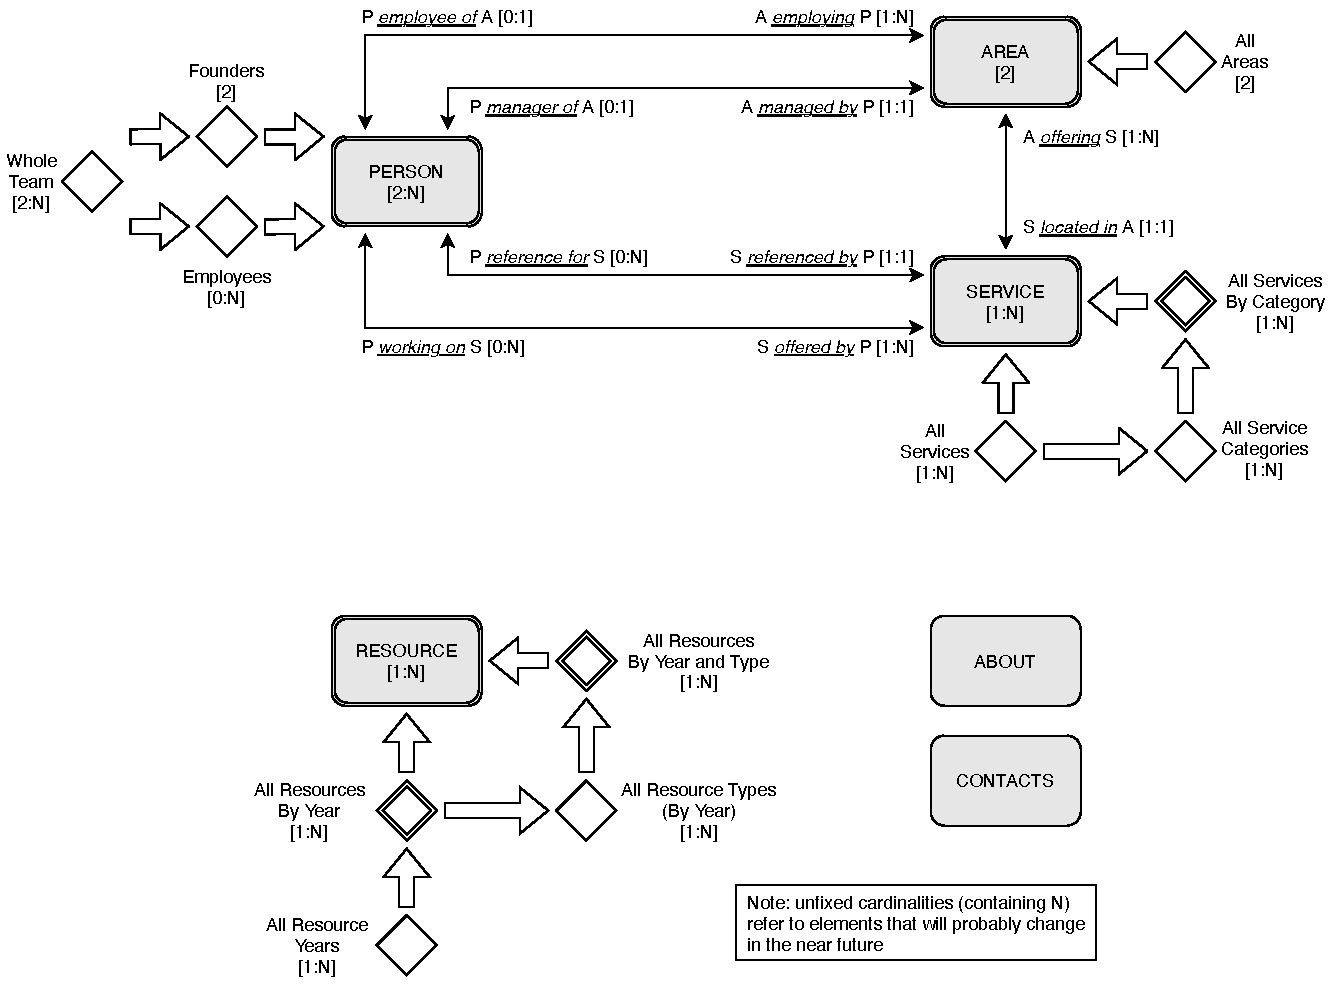
\includegraphics[width=\textwidth]{C-IDM.pdf}
	\caption{C-IDM Diagram}
\end{figure}

\chapter{Content tables}
Here we illustrate the content tables that expand the C-IDM diagram of the previous 
chapter.\\\\
\begin{figure}[h]
	\centering
	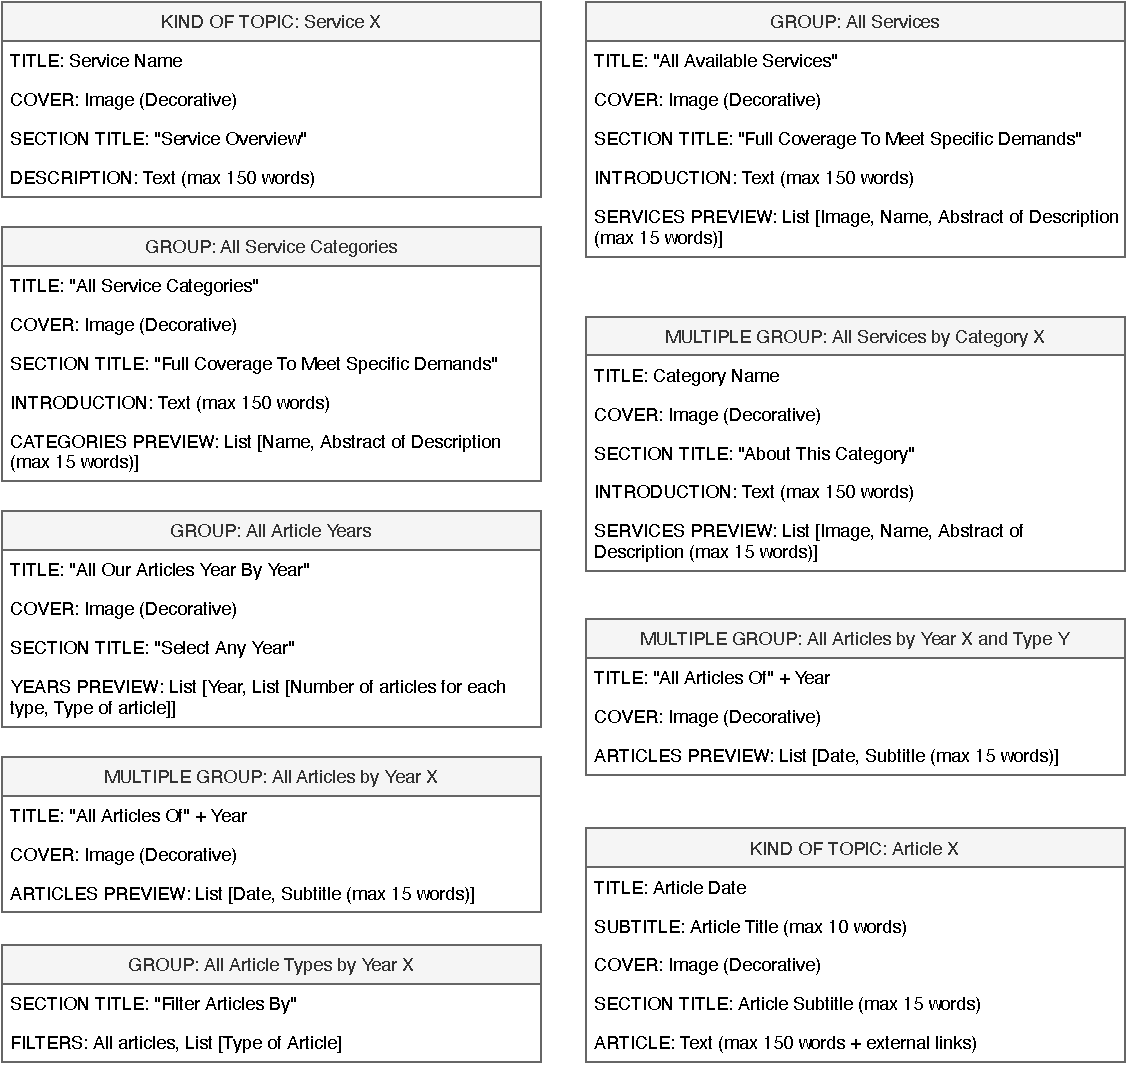
\includegraphics[width=0.9\textwidth]{content_tables_pt2.pdf}
\end{figure}
\begin{figure}[h]
	\centering
	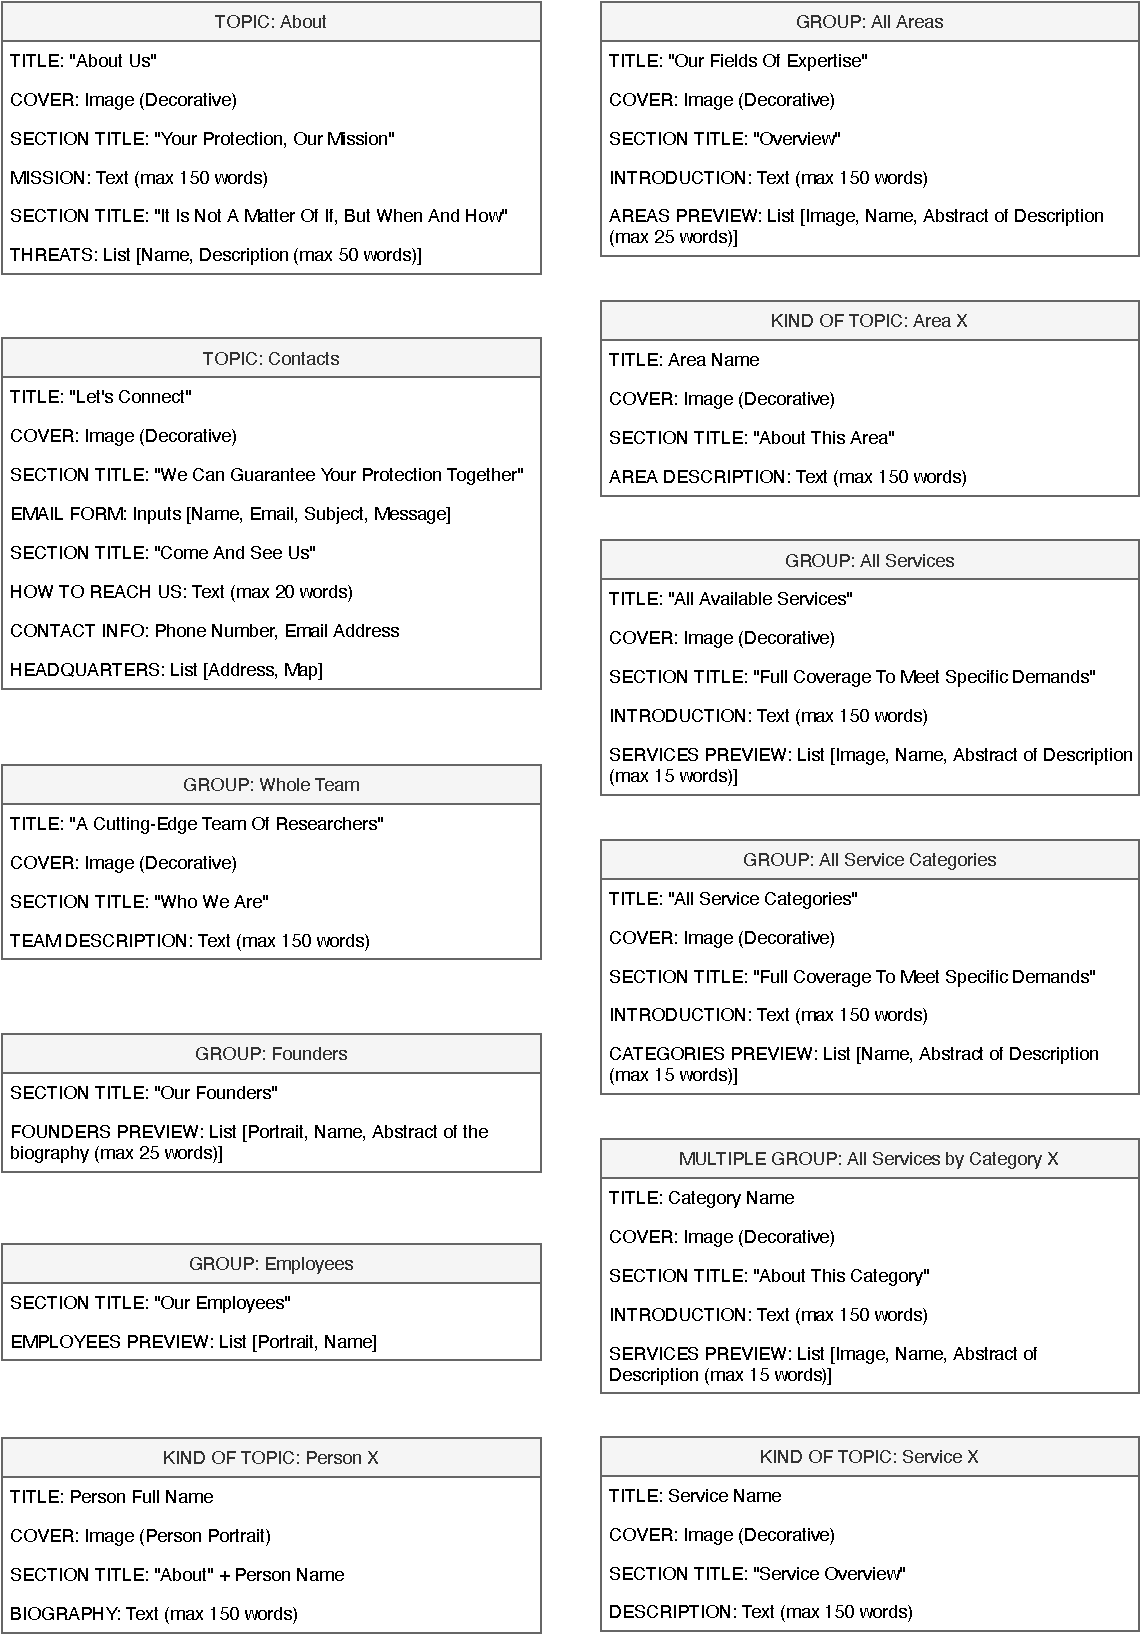
\includegraphics[width=0.9\textwidth]{content_tables_pt1.pdf}
	\caption{Content tables (C-IDM in the small)}
\end{figure}

\chapter{Mapping Content Tables into Pages}
Continuing, we present the result of the application of the process of page mapping 
to the content tables reported in the last chapter. Each table has
been divided into a series of pages, in order to increase the degree of granularity.
\begin{figure}[h]
	\centering
	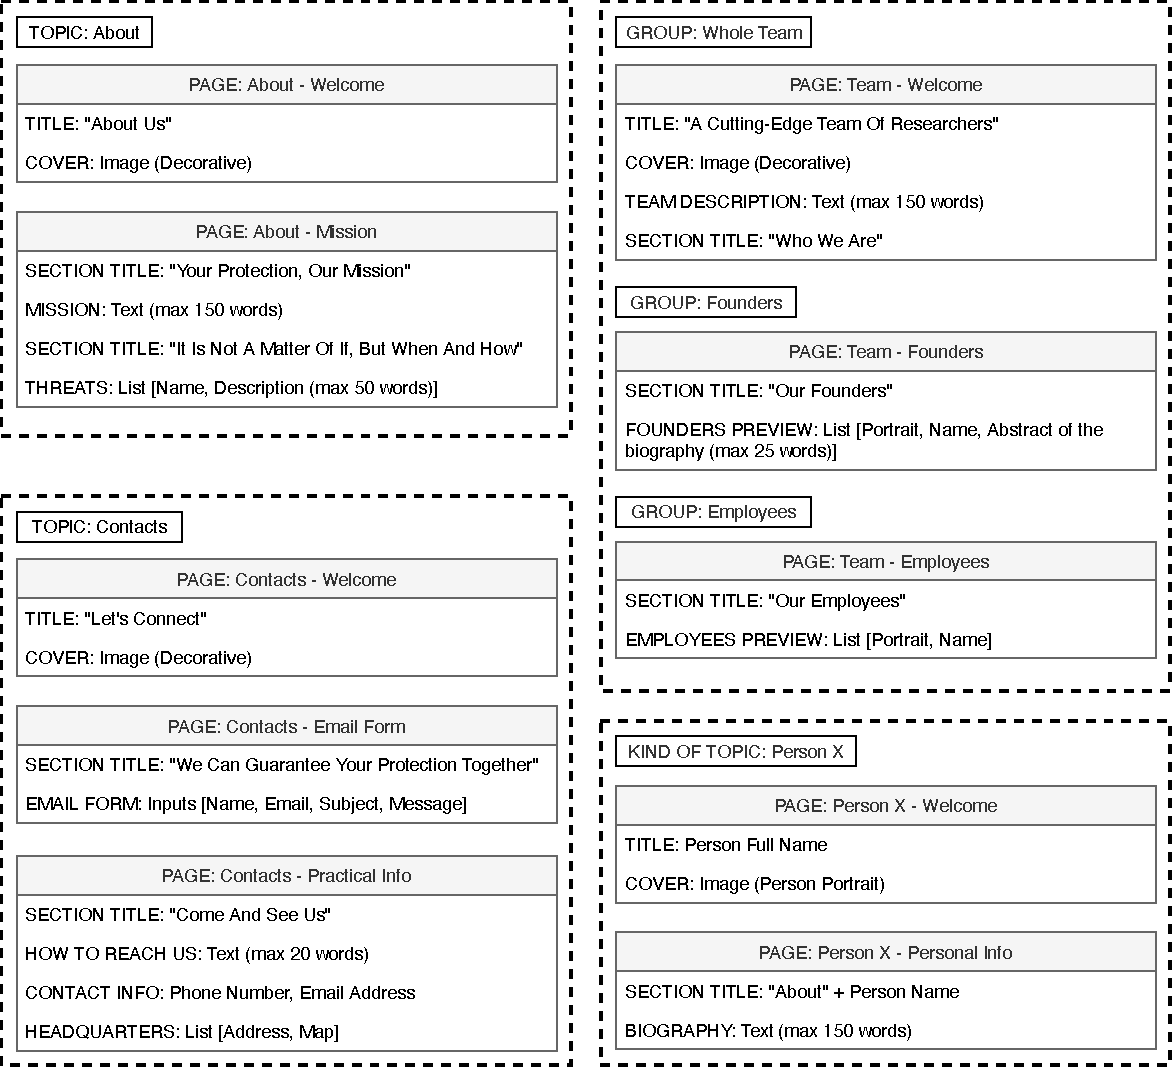
\includegraphics[width=0.95\textwidth]{page_mapping_pt1.pdf}
\end{figure}
\begin{figure}[h]
	\centering
	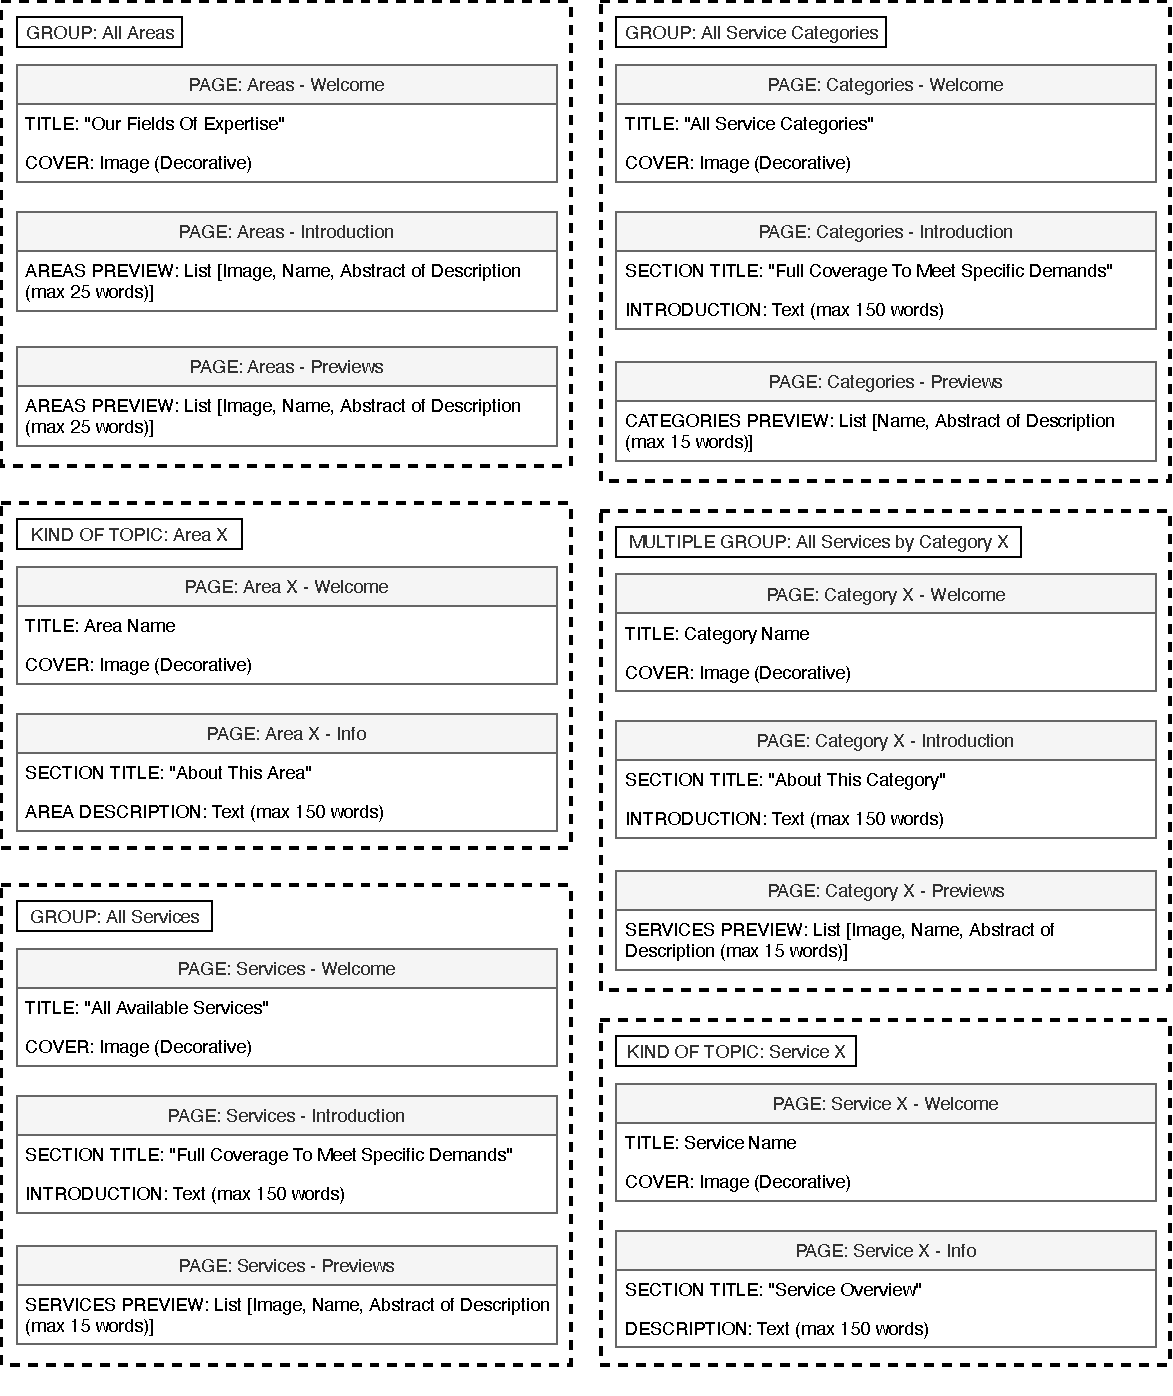
\includegraphics[width=0.95\textwidth]{page_mapping_pt2.pdf}
\end{figure}
\begin{figure}[h]
	\centering
	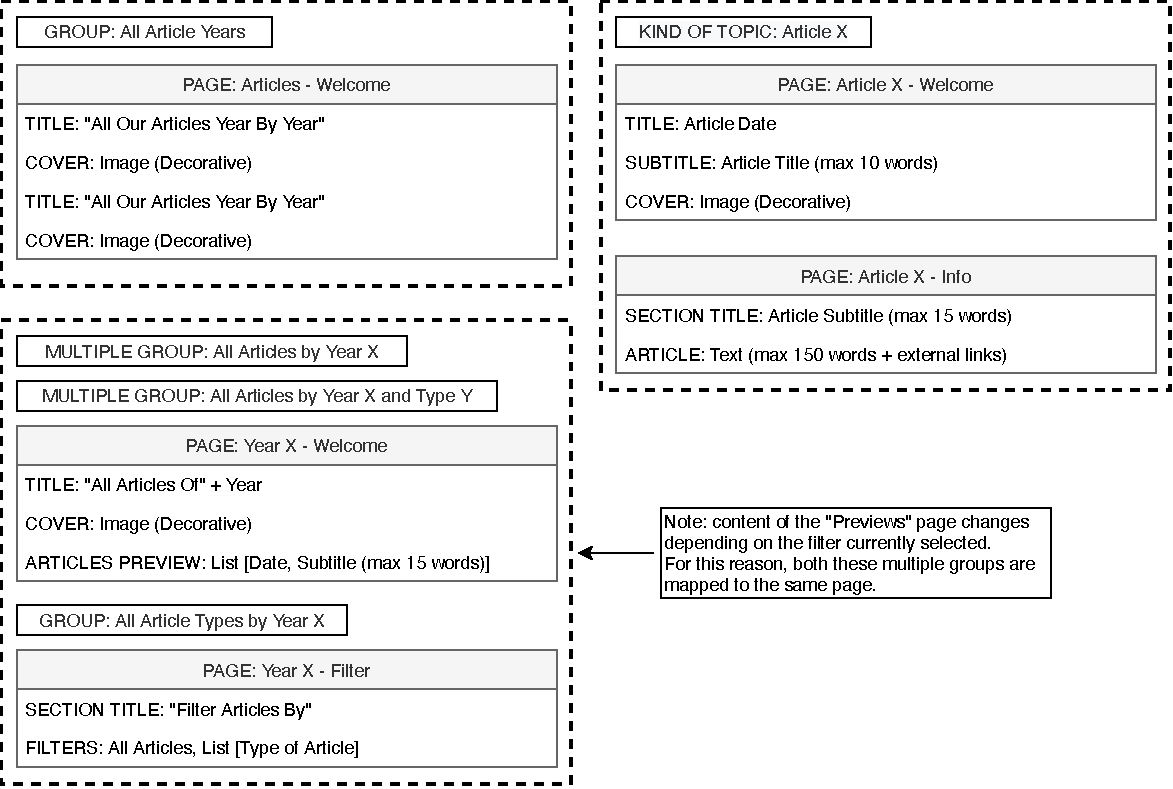
\includegraphics[width=0.95\textwidth]{page_mapping_pt3.pdf}
	\caption{Pages mapping}
\end{figure}

\chapter{P-IDM diagram}
In this section we report the P-IDM diagram which describes the navigation design of our website.\\
\begin{figure}[h]
	\centering
	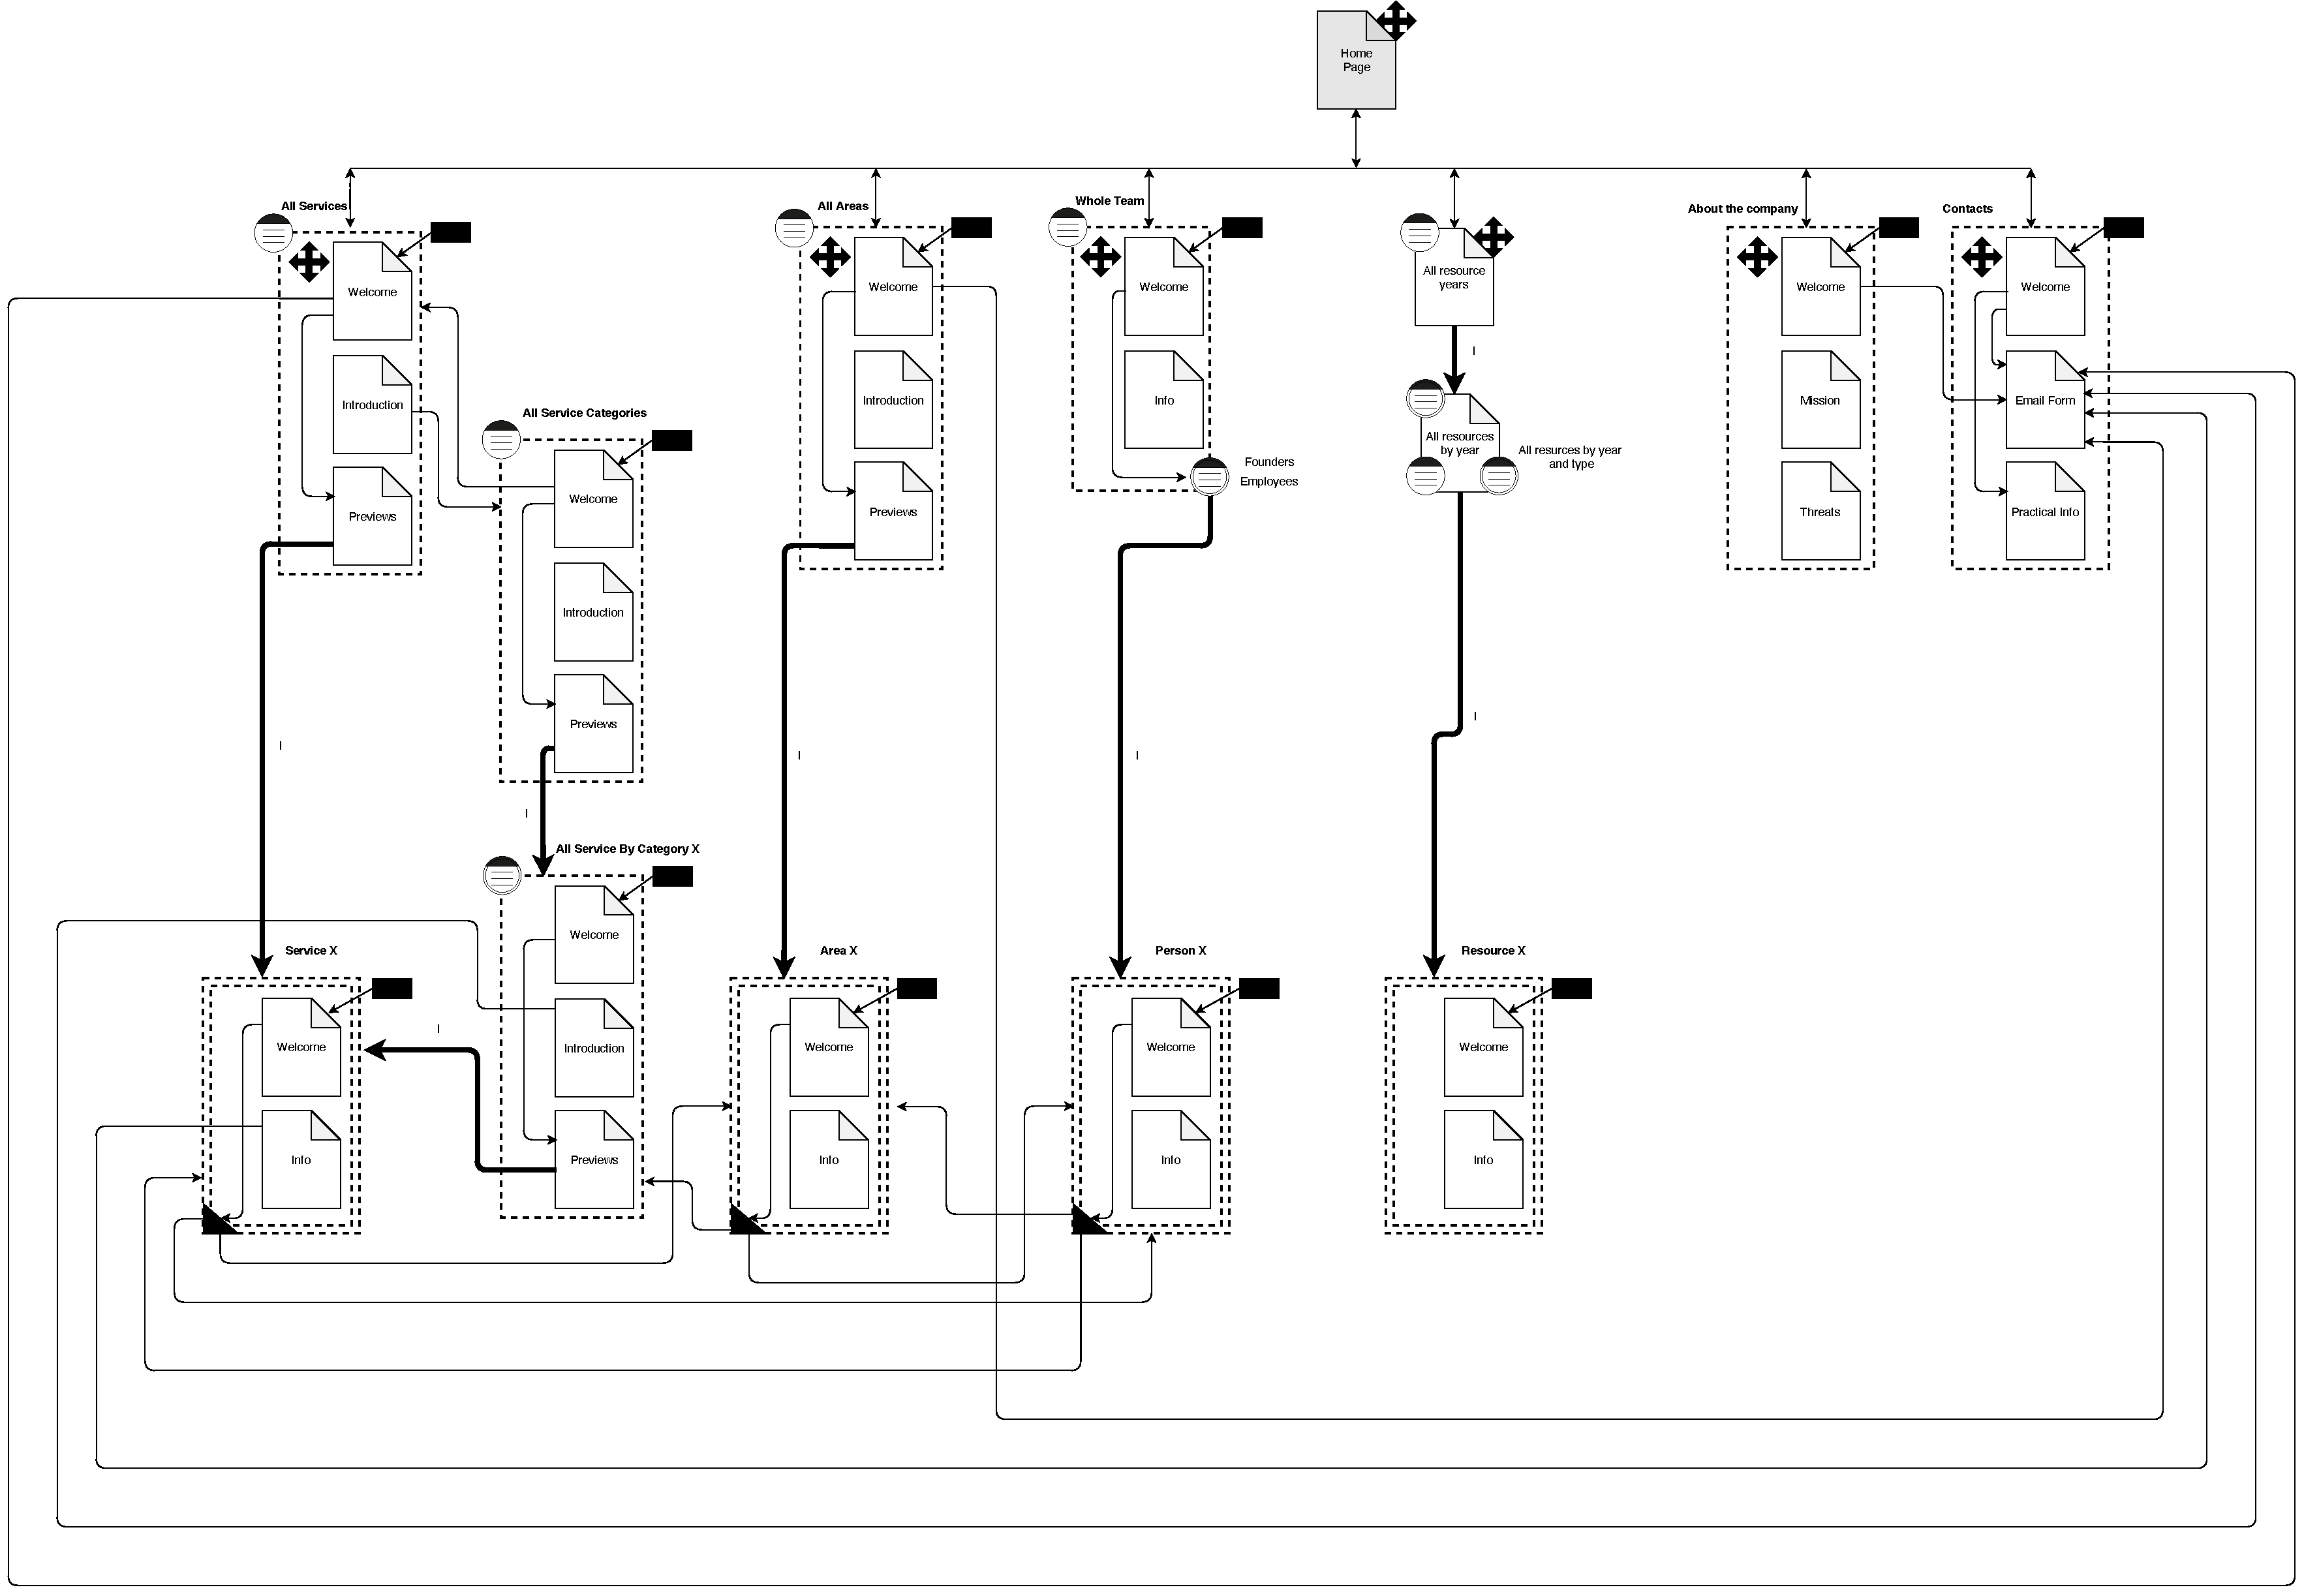
\includegraphics[width=\textwidth]{P-IDM.pdf}
	\caption{P-IDM Diagram}
\end{figure}

\chapter{Visual Design}
Ciao 
%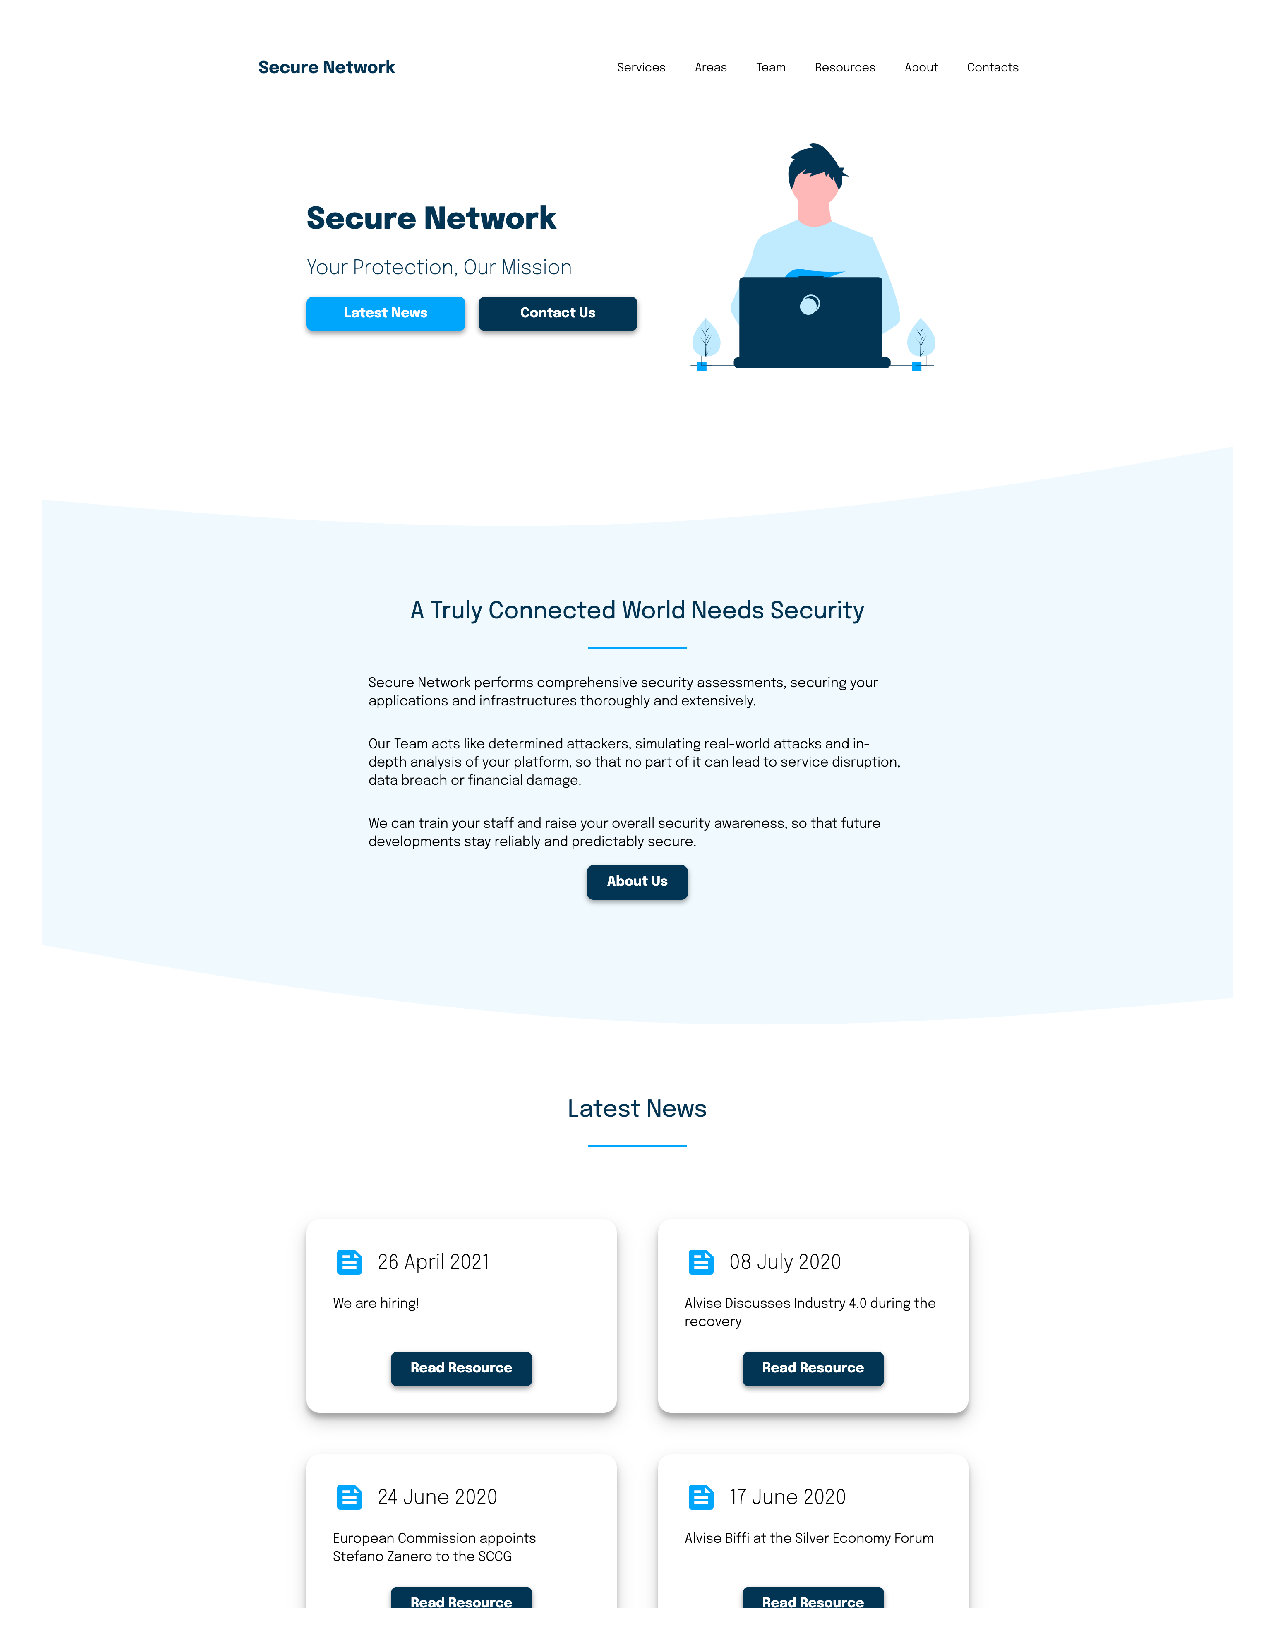
\includepdf[pages=-]{homepage_screen.pdf}




\chapter{Interaction Scenarios}

\chapter{DB Design}
In this last chapter we report the structure of the database designed 
to support the website and manage the information contained in it. 
We started with the conceptual design, by which is possible to identify
the first layer of abstraction of our data. It has been moded with the 
\emph{Entity-Relationship diagram}.\\
\begin{figure}[H]
	\centering
	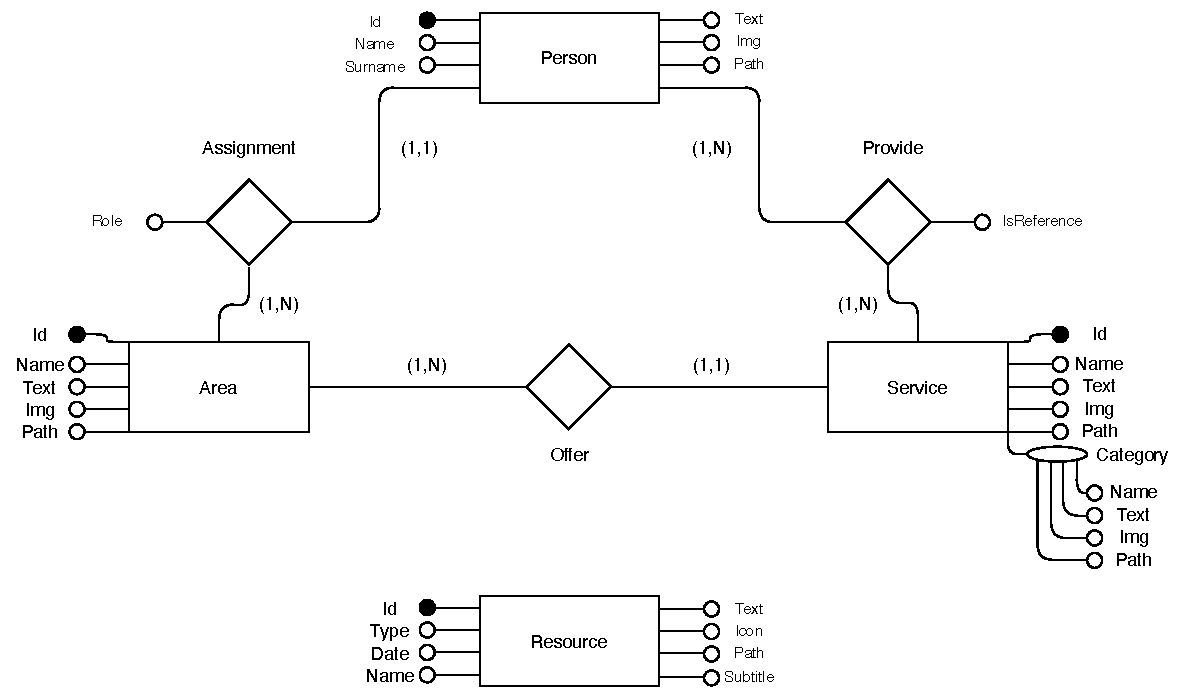
\includegraphics[width=0.95\textwidth]{ER_model.pdf}
	\caption{ER Diagram}
\end{figure}
\noindent
Then we proceed with the logic design, which allow to better describe the
\emph{E-R Model}. Some additional tables have been identified to better 
support the implementation.
\clearpage
\begin{itemize}
	\item \textbf{Area}. An \emph{Area} is identified by an \texttt{id}, 
	has a \texttt{name}, a \texttt{text} description, a string path to the image, 
	\texttt{img}, and a \texttt{path} to reach the specific page. 
	\item \textbf{Person}. A \emph{Person} is identified by an \texttt{id}, 
	has a \texttt{name}, a \texttt{surname}, a \texttt{text} description, a 
	string path to the image, \texttt{img}, a \texttt{path} to reach the specific page.
	In addition, the relation called \emph{Assignment}, among \emph{Person} and \emph{Area}, has
	been merged within the first table, resulting in the addition of two fiels: the 
	\texttt{area\_id} as foreign key and the \texttt{role} of the person within the area.
	Each \emph{Person} is assigned to exactly one \emph{Area}, whereas in each \emph{Area} several
	\emph{People} are assigned.
	\item \textbf{Service\_Category}. This tables was born due to normalization purposes. 
	It would have been redundant adding for each \emph{Service} information about the complex 
	attribute \emph{Category}. To avoid replication, we decided to perform this normalization 
	procedure. A \emph{Service\_Category} is identified by an \texttt{id}, 
	has a \texttt{name}, a \texttt{text} description, a string path to the image, 
	\texttt{img}, and a \texttt{path} to reach the specific page. 
	\item \textbf{Service}. A \emph{Service} is identified by an \texttt{id}, 
	has a \texttt{name}, a \texttt{text} description, a string path to the image, \texttt{img}, 
	a \texttt{path} to reach the specific page.
	The \texttt{category\_id} is the foreign key, used to support the normalization process 
	described in the previous table. 
	Each \emph{Service} is mapped with exactly one \emph{Service\_Category}, whereas each 
	\emph{Service\_Category} is mapped with several \emph{Services}.
	In addition, the relation called \emph{Offer}, among 
	\emph{Service} and \emph{Area}, has	been merged within the first table, resulting in 
	the addition of the fiel \texttt{area\_id} as foreign key.
	Each \emph{Service} is offered by exactly one \emph{Area}, whereas each \emph{Area} offers 
	several \emph{Services}.
	\item \textbf{Person\_Service}. This tables was born to support the \emph{N-N} relation, 
	\emph{Provide}, among \emph{Person} and \emph{Service}. A \emph{Person\_Service} is 
	identified by an autoincremental \texttt{id} and presents a boolean field, \texttt{isReference}, 
	which states whether or not the \emph{Person}, identified by the foreign key \texttt{person\_id}, 
	is the reference for the \emph{Service}, identified by the foreign key \texttt{service\_id}.
	\item \textbf{Resource}. A \emph{Resource} is identified by an \texttt{id}, has a 
	\texttt{type}, a \texttt{name}, a \texttt{date}, a \texttt{text} description, a \texttt{subtitle} 
	a string path to the \texttt{icon}, and a \texttt{path} to reach the specific page. 
\end{itemize}


\begin{figure}[H]
	\centering
	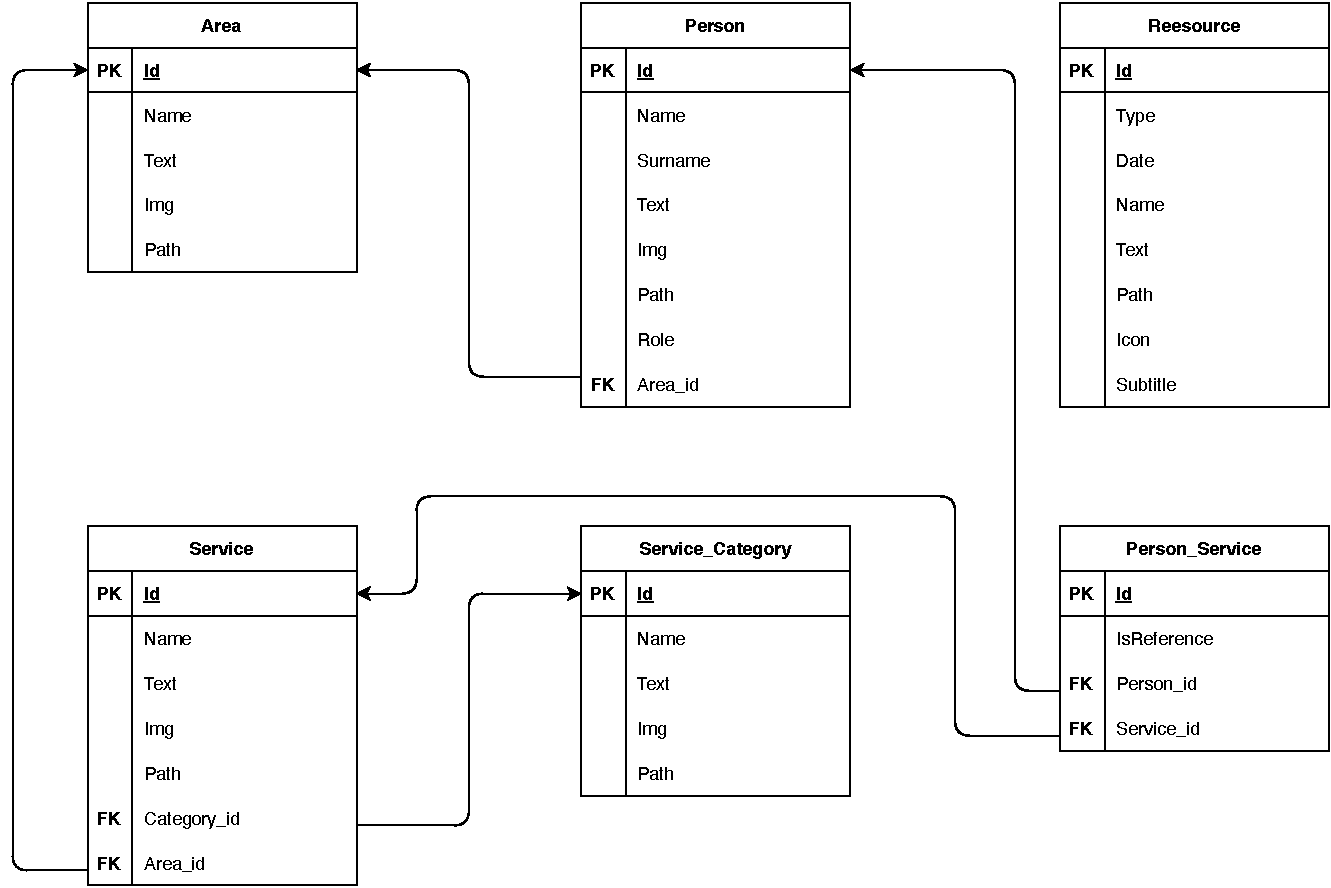
\includegraphics[width=0.95\textwidth]{ER-Logic-Tables.pdf}
	\caption{Relational Tables}
\end{figure}


\listoffigures
\end{document}